\label{chap:pt1_introduction}
In wood industry, finished products are typically obtained through machining processes in which a semi-finished component, such as a wood panel, is processed using a machine known as a \emph{work center}, shown in Fig.~\ref{fig:worktable}.

A typical work center is equipped with a tool storage system from which the tools required to perform operations such as cutting, milling, and contouring on the panel are automatically selected. However, the use of these tools can induce vibrations and oscillations in the workpiece, thereby reducing the quality of the final product~\cite{trappey1990literature,jackson2002waves}. For this reason, keeping the workpiece as stable and firm as possible during machining is crucial.

To support a workpiece during machining, a work center is equipped with a worktable featuring movable bars that translate along the machine’s horizontal axis, above which vacuum suction cup fixtures can be positioned.

The fixtures can be square or rectangular in shape (Fig.~\ref{fig:suction_cups}) and are composed of a square base that allows them to be mounted on the bars and to slide along their length. To improve product quality through an appropriate fixture layout, the fixtures can also be freely rotated to achieve better alignment with the workpiece geometry, with the center of rotation coinciding with the center of the square base.

\begin{figure}[t]
	\centering
	\begin{subfigure}[b]{0.4\textwidth}
		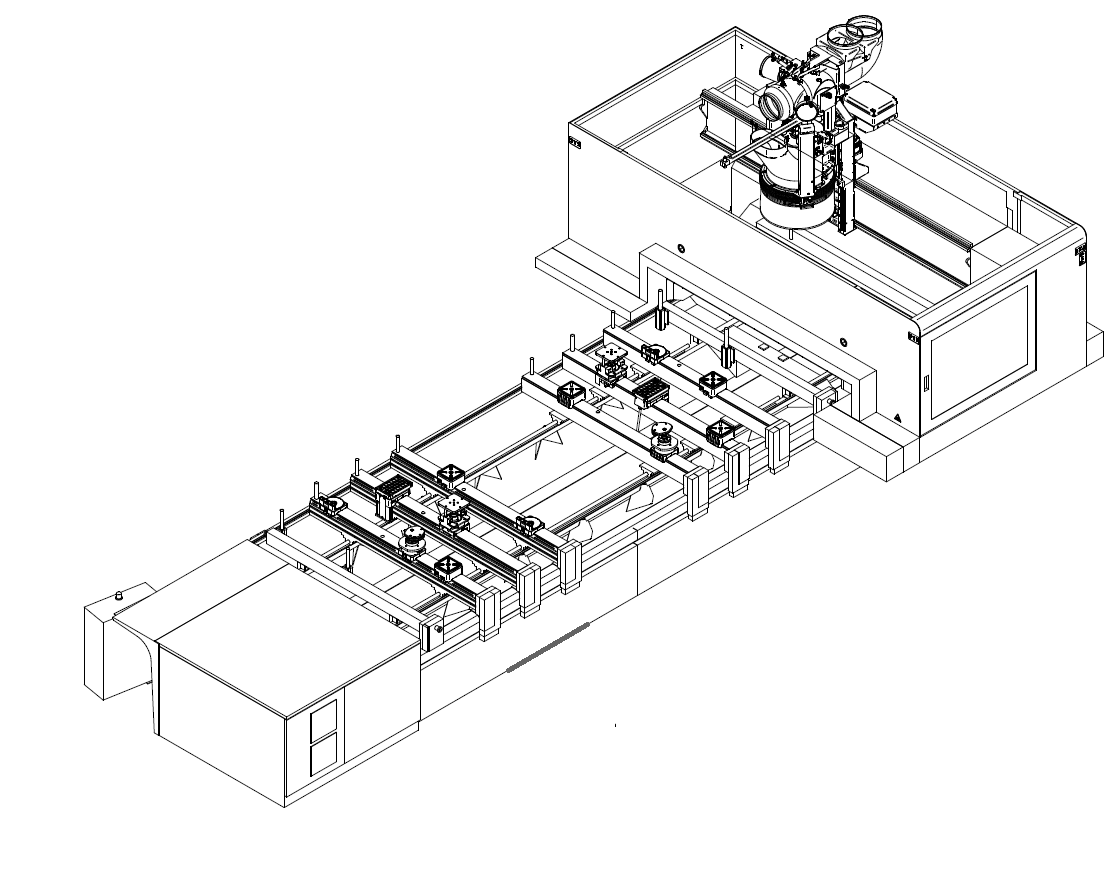
\includegraphics[width=\textwidth]{figures/worktable.png}
		\caption{Work center}
		\label{fig:worktable}
	\end{subfigure}
	\hspace{2cm}
	\begin{subfigure}[b]{0.4\textwidth}
		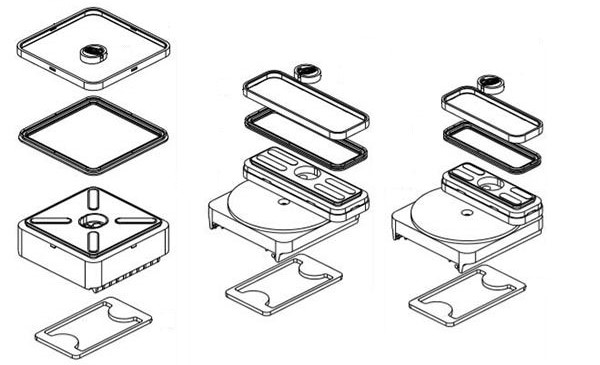
\includegraphics[width=\textwidth]{figures/suction_cups_schema_no_dimnesion.jpg}
		\caption{Vacuum suction cup fixtures}
		\label{fig:suction_cups}
	\end{subfigure}
	\caption{On the left, a work center featuring a worktable with movable bars. On the right, fixtures used to secure the workpiece during machining operations.}
	\label{fig:problem_description_img}
\end{figure}

Determining an appropriate fixture layout for a given workpiece is not always straightforward for a human operator, especially when the workpiece has contoured shapes or includes areas to be extruded. Layouts are often based on the operator’s experience; however, such manually designed solutions are not necessarily optimal and can often be improved by considering the structural properties of the fixtures system, such as its resistance to bending and torsional forces.

The purpose of this work is to determine a sound, and possibly optimal, placement of fixtures under the bottom surface of the workpiece, explicitly accounting for the rotation angle of each fixture.

To solve the problem, we first consider a simplified version that neglects fixture rotation and extrusion areas, addressing it through the formulation of a solver-independent Constraint Programming (CP) model. The performance of the model were evaluated using different solvers and two alternative objective functions: one based on the exact computation of the principal moments of inertia, and the other based on the Manhattan distance between pairs of fixtures.

According to the results obtained and considering more real-world test instances, we revisited the objective function and extended the CP formulation to account for extrusion areas. The performance of the extended CP model were then compared with other solution strategies based on a newly formulated Mixed Integer Programming (MIP) model and a Q-learning based algorithm.

The CP model, the MIP model, and the Q-learning algorithm do not consider fixture rotations, as allowing arbitrary rotation angles significantly increases the number of possible configurations and makes the problem substantially harder to solve. Rotations are subsequently incorporated through a refinement stage based on the Particle Swarm Optimization (PSO) meta-heuristic initialized from the layouts obtained from CP, MIP and Q-learning.

This first part of the thesis is organized as follows. Chapter~\ref{chap:pt1_state_of_the_art} reviews the state of the art. Chapter~\ref{chap:pt1_chapter5} introduces the simplified problem formulation and presents the CP model used to solve it. Chapter~\ref{chap:pt1_chapter6} addresses the complete problem by considering fixture rotations and extrusion areas. Chapter~\ref{chap:pt1_chapter7} analyzes the integration of the proposed solution strategies. Finally, Chapter~\ref{chap:pt1_conclusion} concludes this part of the thesis.
